\documentclass{article}

\usepackage[latin1]{inputenc}
\usepackage{pgfplots}
\usepackage{tikz}
\usetikzlibrary{arrows}

\pgfplotsset{compat=1.10}

\begin{document}
\pagestyle{empty}

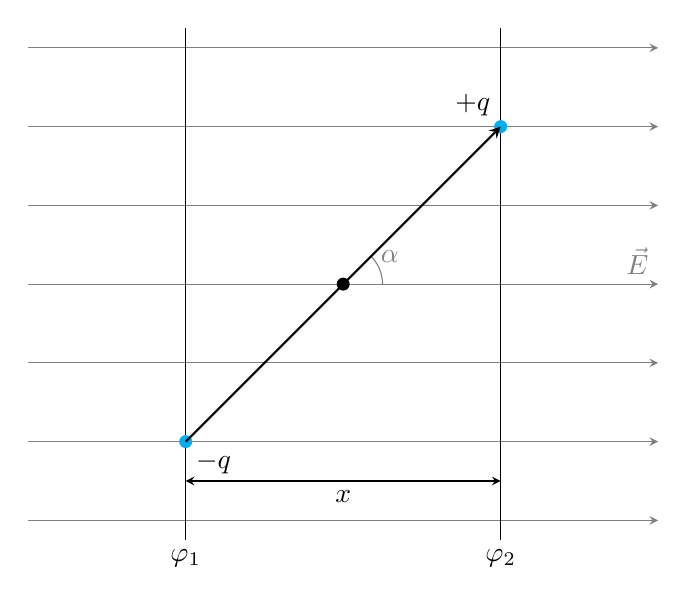
\begin{tikzpicture}[>=stealth]
	\foreach \y in {-3,-2,...,3}
		\draw[-latex, thin, gray, ->] (-4, \y) -- (4, \y);
	\node[gray, above left] at (4, 0) {$\vec{E}$};

	\draw[thin] (-2, -3.25) node[below] {$\varphi_1$} -- (-2, 3.25);
	\draw[thin] (2, -3.25) node[below] {$\varphi_2$} -- (2, 3.25);

	\draw[fill] (0, 0) circle [radius=0.075];

	\draw[gray] (0.5, 0) arc [radius=0.5, start angle=0, end angle=45] node[right] {$\alpha$};

	\draw[<->, thin] (-2, -2.5) -- (2, -2.5);
	\node[below] at (0, -2.5) {$x$};

	\draw[cyan, fill] (2, 2) circle [radius=0.075];
	\draw[cyan, fill] (-2, -2) circle [radius=0.075];
	\draw[-latex, thick, ->] (-2, -2) node[below right] {$-q$} -- (2, 2) node[above left] {$+q$};
\end{tikzpicture}

\end{document}